
\documentclass[11pt,openright,titlepage]{report}


% Configuración page size y márgenes (inner: left, outer: right)
\usepackage[a4paper, inner=3cm, outer=3.25 cm, top=3.25 cm, bottom = 3.5 cm,
            headheight=2cm, voffset=0.5cm, headsep=1.5cm, footskip=1.5cm]{geometry}
            

% Paquetes necesarios o interesantes             
\usepackage[utf8]{inputenc}    % Escribir tildes sin código
\usepackage[english]{babel}    % Escribir en español
\usepackage{graphicx}          % Gráficos 
\usepackage{fancyhdr}          % Personalizar estilo página
%\usepackage{fancyheadings}     % Para los headers y footers (antiguo: no usar, ahora es fancyhdr) 
\usepackage{color}             % Foreground and background color management
\usepackage[usenames,dvipsnames,table]{xcolor}   % Permite modificar tonos de color de forma sencilla
\usepackage{import}            % Importar ficheros de carpetas dentro de este proyecto
\usepackage{listings}          % Permite pegar texto sin formato. Específico para pegar código
\usepackage{placeins}          % Float barriers para imágenes/tablas/etc
\usepackage{float}             % Usar [H] para tablas
\usepackage{amsmath}           % Fórmulas matemáticas
\usepackage{verbatimbox}       % Encuandrar en cajas texto sin formato (verbatim)
\usepackage{background}        % Personalizar background 
\usepackage{tikz}              % Para graficar desde latex
\usepackage{tikz-qtree}        % Para dibujar esquemas en forma de árbol
\usepackage{tgadventor}        % Sans serif font   
\usepackage{charter}           % Serif font           
\usepackage{tgtermes}          % Serif font
\usepackage{tgpagella}         % Serif font
\usepackage{soul}              % Para separar con guiones las palabras cuando no caben en la línea de texto
\usepackage{titlesec}          % Select alternative section titles
\usepackage{hyperref}          % Vínculos


% Colores adicionales
\definecolor{codegreen}{rgb}{0,0.6,0}
\definecolor{codegray}{rgb}{0.5,0.5,0.5}
\definecolor{codepurple}{rgb}{0.58,0,0.82}
\definecolor{backcolour}{rgb}{0.95,0.95,0.92}
\definecolor{darkBlue}{RGB}{0,0,120}


% Configuración de los hipervínculos
\hypersetup{
     colorlinks   = true,
     citecolor    = gray,
     urlcolor     = CadetBlue,
     linkcolor    = darkBlue,
     %linktoc      = all
}


  %Header
\pagestyle{fancy}
\fancyhead{} % get rid of headers
\renewcommand{\headrulewidth}{0pt}
\newcommand{\changefont}{\fontfamily{qag}\selectfont}
\rhead{\changefont{The USB \\ Mopta 2017 competition}} 
% Para las páginas con \chapter
\fancypagestyle{plain}{
\fancyhead{} % get rid of headers
\rhead{\changefont{The USB \\ Mopta 2017 competition}}
}


  %Formato de títulos des capítulos, secciones, etc
\titleformat{\chapter}
 {\LARGE\fontfamily{qag}\selectfont\bfseries\color{Bittersweet}}{\thechapter. }{0pt}{}
\titleformat{\section}
{\color{BurntOrange}\Large\fontfamily{qag}\selectfont\bfseries}
{\color{BurntOrange}\thesection}{1em}{}
\titleformat{\subsection}
{\color{BurntOrange!85!}\large\bfseries}
{\color{BurntOrange!85!}\thesubsection}{1em}{}
\titleformat{\subsubsection}
{\color{BurntOrange!85!}\normalsize\bfseries}
{\color{BurntOrange!85!}\thesubsubsection}{1em}{}

 
 % Para códigos
\lstdefinestyle{mystyle}{
    backgroundcolor=\color{backcolour},   
    commentstyle=\color{codegreen},
    keywordstyle=\color{magenta},
    numberstyle=\tiny\color{codegray},
    stringstyle=\color{codepurple},
    basicstyle=\footnotesize,
    breakatwhitespace=false,         
    breaklines=true,                 
    captionpos=b,                    
    keepspaces=true,                 
    numbers=left,                    
    numbersep=5pt,                  
    showspaces=false,                
    showstringspaces=false,
    showtabs=false,                  
    tabsize=2
}
 
\lstset{style=mystyle}


%  CONFIGURACIÓN DEL DOCUMENTO

\begin{document}

% Importa la portada
%\import{pages/}{PortadaClientes.tex}


%\fontfamily{qag}\selectfont   % TEX Gyre Adventor        
\fontfamily{bch}\selectfont    % charter           


% Crea la tabla de contenidos
\SetBgContents{}
\pagenumbering{gobble}
% Los vínculos de la tabla serán negros
\hypersetup{linkcolor=black} 
%\tableofcontents\clearpage
% El resto de vínculos serán azules
\hypersetup{linkcolor=darkBlue}

% Crea el logo en la esquina derecha - baobab
\SetBgScale{1}
\SetBgAngle{0}
\SetBgOpacity{1} 
\SetBgHshift{8cm}
\SetBgVshift{12.6cm}
%\SetBgContents{\includegraphics[width=1.1cm,scale=0.2]{imagenes/arbol_baobab.jpg}}
% Crea el logo en la esquina izquierda - cliente
%\SetBgScale{1}
%\SetBgAngle{0}
%\SetBgOpacity{1} 
%\SetBgHshift{-7cm}
%\SetBgVshift{12.6cm}
%\SetBgContents{\includegraphics[width=1.1cm,scale=1.0]{imagenes/LogoCliente.png}}

% Footer
\let\oldfootnotesize\footnotesize
\renewcommand*{\footnotesize}{\oldfootnotesize\scriptsize}
% Empieza a contar desde 1
\setcounter{page}{1}
\renewcommand{\thepage}{\arabic{page}}

% Importar las secciones del documento. Ejemplo:
%\import{Pages/}{MiFichero.tex}

\chapter{Introduction}

This document has as purpose the explanation of the concepts in the problem presented in the MOPTA challenge, the methodology, techniques and assumptions used to implement a model and the mathematical implementation of said model.

In order to understand this document, it is necessary to first read and understand the problem at hand. The problem consists on a logistics and production problem where the product quality decays over time. This has implications such as that there are lower and upper limits for the time that needs to pass between production and consumption. Routing also needs to be used to transport efficiently the products between nodes.

More detail about the problem can be found in the \href{http://coral.ie.lehigh.edu/~mopta/AIMMS_MOPTA_case_2017.pdf}{following document}.

This document contains three chapters. In the first one, some definitions are made about production, transportation and demand as well as some grouping assumptions of these.

Te second chapter focuses on the Mathematical Formulation for the model that solves and returns a solution for this problem.

Finally, a summary of the tests that were done and a brief representation of a solution.

\chapter{Definitions}
\label{def}

 %TODO: insert graphs.

Following are several concepts related to the problem at hand. These terms will be later referenced in the model section (section \ref{matmod}.

\section{Production}

\subsection{Production line and type}
\label{def:lines}

A production line consists on each of the places where production can happened. Each line works independently from the other an are identical in their capacity to produce.

They have an associated cost to be used at least once during the day.

There exists a definite set of production "`drives"' that a line can be in. They have been called "`production types"'. Each type consists on a combination of three parameters:

\begin{itemize}
	\item Time to produce.
	\item Number of dosages to produce.
	\item Radioactivity level of dosages when produced.
\end{itemize}

Each line can produce any of these production types and can change from producing one type to producing the other without any extra cost.

\subsection{Production job}

A production job consists of a given batch of dosages produced at a specific production line.

It is represented by a tuple with numbers. The first one is the production line it belongs, the second is a correlative number.

Jobs are defined in advance so that each production line has a number of candidate jobs available to potentially use.

Also, each job needs to have assigned a "job type" (see \ref{def:lines} for more information).

\subsection{Job-Job type}

In order to reduce the size of the problem and break the symetry on the decision variables, each production line can produce only certain types of jobs. For example, the first production line can produce only the first two types of jobs.

We thus sacrifice optimality (we reduce some possibilities) in order not to have too many decision variables.

The maximum number of jobs per line also depends on which types of jobs the line can do. It is assumed that a line that only has particularly long-duration job types available will not do many jobs.

\section{Demand}

\subsection{Center}

Each center is a physical place where dosages are consumed during the day. There are both distances and times between each center. These distance and times matrices are considered to be symmetrical.

Each center has, in addition, a specific time to unload the dosages once the vehicle arrives.

During the model formulation, centers can also be called nodes.

\subsection{Clustering of centers}
\label{def:cluster}

Due to the number of combinations of possible routes (see section \ref{def:route}) that any vehicle can do, centers have been grouped into groups (or clusters).

The clustering of centers has been achieved with a K-means algorithm using the distance matrix between centers. The production center has not been included in the clustering procedure given that this center will be included in every cluster.

\subsection{Patient}

Patients are represented as dosages that need to be administered in a given center and on a specific time.

More generally, we define a patient as a number of dosages that need to be administered between a minimum and a maximum time. 

A particular case of this formulation would be to treat each appointment as a patient. In this case, the patient would have a dosage of 1 and a minimum time equal to the maximum time.

It is defined as a tuple of two numbers. The first one is the center to which the patient belongs, the second one is the correlative number of patient in the day.

\section{Transport}

\subsection{Vehicle}

A vehicle is the means for transporting dosages between the production node and each of the centers. They need to do specific routes between each center in order to arrive on time for each patient's appointment.

There is a finite number of vehicles, all identical. There is no capacity limit on the amount of dosages each vehicle can take in total and the the cost of the vehicle has three components:

\begin{itemize}
	\item Total distance traveled.
	\item Total time traveled.
	\item Usage of vehicle.
\end{itemize}

\subsection{Route}
\label{def:route}

A route is the specific travel of a single vehicle.

It is defined by a tuple with two numbers. The first one is the vehicle that can do the route, the second one is the correlative number of route of that specific vehicle.

Routes are pre-calculated, so each vehicle has the following information:

\begin{itemize}
	\item The number of routes it can do.
	\item The centers the route has to visit, in case of being activated.
\end{itemize}

\subsection{Cluster-route}

In order to assign groups of centers to vehicles, a clustering of centers has been made. The number of clusters depends on the total number of vehicles and centers available. See section \ref{def:cluster}.

Each route, when active, needs to visit each one of the centers in the cluster. In a sense, it behaves similarly to a Travelling Salesman Problem with time windows.

Given the clustering of centers explained in section \ref{def:cluster}, not all vehicles can visit all centers. Dependind on the configuration adopted and the number of vehicles and centers, each vehicle will be able to visit between 1 and 3 clusters. 

Furthermore, each specific route of a vehicle (see section \ref{def:route}) will only be able to visit 1 cluster. The idea is to have many different vehicles capable of servicing the same cluster. This way it is possible to reduce the number of vehicles if necessary without compromising feasibility.
\chapter{Mathematical formulation}

The model is essentially an assignment problem where each patient gets assigned a vehicle's route and a production job.

\section{Production job}

A production job consists of a given batch of dosages produced at a specific production line.

It is represented by a tuple with numbers. The first one is the production line it belongs, the second is a correlative number.

Jobs are defined in advance so that each production line has a number of candidate jobs available to potentially use.

Also, each job needs to have assigned a "job type" (see FALTA for more information).

In order to reduce the size of the problem and break the symetry on the decision variables, each production line can produce only certain types of jobs. This way, the first production line can produce only the first two types of jobs.

The maximum number of jobs per line also depends on which types of jobs the line can do. It is assumed that a line that only has particularly long job types available will not do many jobs.

\section{Patient}

Patients are represented as dosages that need to be administered in a given center and on a specific time.

More generally, we define a patient as a number of dosages that need to be administered between a minimum and a maximum time. 

A particular case of this formulation would be to treat each appointment as a patient. In this case, the patient would have a dosage of 1 and a minimum time equal to the maximum time.

It is defined as a tuple of two numbers. The first one is the center to which the patient belongs, the second one is the correlative number of patient in the day.

\section{Route}

A route is the specific travel of a single vehicle.

It is defined by a tuple with two numbers. The first one is the vehicle that can do the route, the second one is the correlative number of route of that specific vehicle.

Routes are pre-calculated, so each vehicle has the following information:

* The number of routes it can do.
* The centers the route has to visit, in case of being activated.

In order to assign groups of centers to vehicles, a clustering of centers has been made. The number of clusters depends on the total number of vehicles and centers available. See section \ref{clusters}.

Each route, when active, needs to visit each one of the centers in the cluster. In a sense, it behaves similarly to a Travelling Salesman Problem with time windows.

\subsection{Clusters of centers}
\label{clusters}

The clustering of centers has been achieved with a K-means algorithm using the distance matrix between centers. The production center has not been included in the clustering procedure.

\section{Sets}

* Production lines: each production line that can be used to produce dosages.
* Job types: each one of the different ways that dosages can be produced.
* Vehicles: each transport that can be used simmultaneously to take dosages from the production center to the demand centers.
* Centers: each of the physical locations where dosages are applied to patients.
* Jobs: each production batch that is done at every production line. Each job has only one job type.
* Routes: each of the travels that every vehicle does when being used.
* Patients: each of the patients that needs dosages.

\begin{tabular}{p{15mm}lp{105mm}}
    $\mathcal{L}$    & : & all production lines \\
    $\mathcal{T}$    & : & all job types \\                    
    $\mathcal{V}$    & : & all vehicles \\    
    $\mathcal{C}$    & : & all centers \\    
    $\mathcal{J}$    & : & all jobs \\    
    $\mathcal{R}$    & : & all routes \\    
    $\mathcal{P}$    & : & all patients \\
\end{tabular}
\bigskip

\section{Decision variables}

\subsection{Production variables}

\begin{tabular}{p{15mm}lp{105mm}}
    $lineUsed_{l}$    & : & 1 if line $l \in \mathcal{L}$ will be used  \\  
    $jobUsed_{j}$    & : & 1 if job $j \in \mathcal{J}$ will be used  \\  
    $jobType_{jt}$    & : & 1 if job type $t \in \mathcal{T}$ is assigned to job $j \in \mathcal{J}$ \\  
    $jobST_{j}$    & : & minute at which the job $j \in \mathcal{J}$ starts \\  
%    $jobProd_{j}$    & : & minute at which the job $j \in \mathcal{J}$ starts \\  
%    $jobTime_{j}$    & : & minute at which the job $j \in \mathcal{J}$ starts \\  
\end{tabular}
\bigskip

\subsection{Transport variables}

\begin{tabular}{p{15mm}lp{105mm}}
    $routeUsed_{r}$    & : & 1 if route $r \in \mathcal{R}$ will be used  \\  
    $vehicleUsed_{v}$    & : & 1 if vehicle $v \in \mathcal{V}$ will be used  \\  
    $routeArrival_{rc}$    & : & minute at which route $r \in \mathcal{R}$ arrives to center $c \in \mathcal{C}$ \\  
    $routeST_{r}$    & : & minute at which the route $r \in \mathcal{R}$ starts \\
    $routeArc_{rcc'}$    & : & 1 if route $r \in \mathcal{R}$ visits center $c'$ inmediately after center $c'$  \\
    $routeET_{r}$    & : & minute at which the route $r \in \mathcal{R}$ finishes \\
\end{tabular}
\bigskip

\subsection{Demand variables}

\begin{tabular}{p{15mm}lp{105mm}}
    $routeJobPatient_{rjp}$    & : & 1 if route $r$ will be used to transport a dosage from job $j$ to patient $p$ \\  
    $routeJob{rj}$    & : & 1 if route $r$ is used to transport dosages for job $j$ \\  
    $jobPatient_{jp}$    & : & 1 if job $j$ is used to produce dosages for patient $p$ \\  
    $routePatient_{rp}$    & : & 1 if route $r$ is used to transport dosages for patient $p$\\
\end{tabular}
\bigskip



\chapter{Results}
\label{results}

Different experiments have been done and stored. Below, a list of criteria for the creation of experiments is explained and a table with results for each experiment is presented.

\section{Control parameters}

The following is a list of parameters used to define different experiments.

\paragraph{Number of centers}

This parameter conditions the size of the real problem. It was made to test the model with smaller-size problems.

\paragraph{Patients' period size}

This parameter is a very important one. It groups appointments into patients (see \ref{sec:patients}) and it can do so in one of the following options (in minutes): "`No grouping"', 30, 60, 90, 120.

\paragraph{Solver}

Two solvers have been used: GUROBI and CBC. From the experiments, CBC was able to find feasible and reasonably good solutions for instances of less than 7 centers. GUROBI performed a lot better, as expected.

\paragraph{Solving time}

The following options of solving times were tried, in seconds: 25000, 40000.

\paragraph{Number of routes per vehicle}

The maximum number of routes that a vehicle can make. Values ranged between 2 and 4.

\paragraph{Other assumptions}

There was additional configuration that was tested during the development and construction of the model with small instances. It was not part of the experimentation process but does condition the quality of the solutions.

They are the following:

\begin{itemize}
	\item \textbf{Number of jobs per line}: 3, 5, 7, ..., 3 + 2 * (number of lines -1).
	\item \textbf{Total number of vehicles}: kept a the maximum.
	\item \textbf{Total number of lines}: kept at the maximum.
\end{itemize}

\section{Experiments}

Below are the results from the experiments that were run by doing changes in the parameters presented above.
Some of the parameter were not saved for some of the executions, like the solving time.


The best results were obtained when grouping patients into 60-minute blocks and 90-minute blocks. Using 2 routes per vehicle sometimes helped obtain a faster solution but not necessarily was better. Solving time was not highly relevant since the reduction on the gap was not significative.


The best gaps that were obtained got around 20\% and 40\%. None of the big instances was solved up to optimality.

\begin{center}
\begin{tabular}{c|c|c|c|c|c|c|c}
Experiment    & Solving  &  Period  &    Solver   &   Routes per &Centers &  Cost       &   GAP   \\
              & Time     &          &             &    vehicle   &        &             &   (\%)   \\ \hline
201705070923  & 25000         &  30      &    GUROBI   &   2          &  8     &  21132      &       \\ \hline
201705071205  &  5000         &  30      &    GUROBI   &   4          &  8     &  21432      &       \\ \hline
201705071948  & 25000         &  30      &    GUROBI   &   4          &  8     &  21432      &       \\ \hline
201705080316  & 25000         &  90      &    GUROBI   &   4          &  8     &  18438   &  23.1    \\ \hline
201705090800  & 40000         &  30      &    GUROBI   &   4          &  8     &  18738   &  36.1     \\ \hline
201705212256  & 3000          &  60      &    CBC      &   4          &  4     &  11359   &       \\ \hline
201705220557  & 25000         &  60      &    CBC      &   4          &  8     &  30617    &  208    \\ \hline
201705230608  & 25000         &  60      &    GUROBI   &   2          &  8     &  18482    &  31.5    \\ \hline
201705021351  &               &  30      &    GUROBI   &   2          &  3     &  12478   &       \\ \hline
201705021437  &               &  60      &    GUROBI   &   2          &  3     &  12478   &       \\ \hline
201705021554  &               & 120      &    GUROBI   &   2          &  8     &  18911   &       \\ \hline
201705070048    &             & None     &  GUROBI      &   4           &   8   &   30208 &      \\ \hline
201705070150    &               &   60      &   GUROBI  &   4           &   8   &   21732    &          \\ \hline
201705081624   & 25000         &   120      &   GUROBI  &   4           &   8   &   20538    &  32.5 \\ \hline
201705091923   & 40000         &   None      &   GUROBI  &   4           &   8   &   19974    &  50.5 \\ \hline
201706190051   & 40000         &   60      &   CBC  &   2           &   8   &   23909    &  100 \\ \hline
    \end{tabular}
\end{center}

\subsection{Solution}

As an example of how the solution is interpreted, a graph has been produced in figure \ref{fig:solution} to show the production and routing in one of the cases. The case being shown is "`201705230608"'.

The graphs assumes that time = 0 equals 7:00 AM in the morning.

In the first rows (production lines), identified with the name "`Line X"' the following is true:

\begin{itemize}
	\item colors mark the job type.
	\item tasks mark production jobs.
\end{itemize}

In the following rows (vehicles), identified with the name "`Vehicle X"' the following is true:

\begin{itemize}
	\item each color is the center from where vehicle exits (red is the production node).
	\item each task is the duration of the trip of the vehicle.
\end{itemize}

\begin{figure}
	\centering
		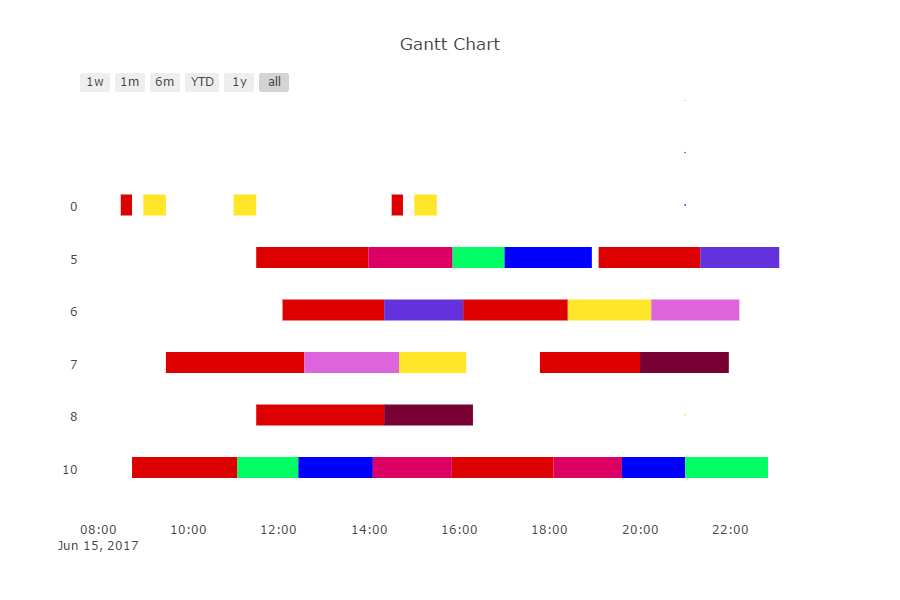
\includegraphics[width=\textwidth]{imagenes/production_and_routes.png}
	\caption{Production and routing}
	\label{fig:solution}
\end{figure}


%\include{pages/ModeloEstadistico}

\end{document}
